%% Supplementary Information for the Torddis manuscript
%% Content moved out of the main manuscript for length/relevance reasons.

\section{Test Cases Used in Acceptance Testing}
\label{sup:test-cases}
This supplementary section presents the acceptance test cases that were designed and executed during the Torddis system development, following ISO/IEC/IEEE~12207 and TDDM4IoTS practices.



\section{Review of AI Methods for Distraction Monitoring}
\label{sup:ai-methods}
This supplementary section reviews the AI methods surveyed during the preliminary analysis of the Torddis project. Tables list facial-recognition, facial-expression, drowsiness-detection and object-recognition methods evaluated in the literature.

\subsubsection{AI Methods for Monitoring Children's Distractions}
                In this stage, the most suitable AI methods were selected to implement the Torddis proposal. These include methods for:
                
                \begin{itemize}
                    \item Facial recognition,
                    
                    \item Facial expression recognition,
                    
                    \item Drowsiness detection, and
                    
                    \item Object recognition.
                \end{itemize}
                
                \paragraph{Facial Recognition Methods.}
                Facial recognition methods focus on face detection by identifying patterns such as eyes, lips, mouth, and nose, among other facial features. Table \ref{tab:facial-recognition} lists several methods used for face detection and recognition.
                
                \begin{table}[!htbp]
                    \caption{Facial recognition methods}
                    \label{tab:facial-recognition}
                    \centering
                    {\footnotesize
%
                        \begin{tabular}{
                                >{\raggedright\arraybackslash}p{0.25\textwidth}
                                >{\raggedright\arraybackslash}p{0.20\textwidth}
                                >{\raggedright\arraybackslash}p{0.45\textwidth}
                                >{\raggedright\arraybackslash}p{0.10\textwidth}
                            }
                            \toprule
                            \textbf{Method} &
                            \textbf{Implementation Environment} &
                            \textbf{Purpose} &
                            \textbf{Accuracy} \\
                            \midrule	
                            HCC\textsuperscript{a} & OpenCV & Face detection in low-light environments \citep{Le2022Facial}. & \multicolumn{1}{r}{81.00\%} \\								
                            
                            & \textit{(not specified)} & Gender classification \citep{Goel2012Hybrid}. & \multicolumn{1}{r}{98.75\%} \\
                            
                            Amazon Rekognition & AWS\textsuperscript{b} & Authentication through facial recognition \citep{Girmay2021AI}. & \multicolumn{1}{r}{100\%} \\
                            
                            YOLO\textsuperscript{c}, MTCNN\textsuperscript{d}, and FaceNet with SVC\textsuperscript{e} & Google Colab & Attendance registration based on deep learning \citep{Darapaneni2020Automatic}. & \multicolumn{1}{r}{99.00\%} \\
                            
                            LBPH\textsuperscript{f} & \textit{(not specified)} & Facial detection from captured images \citep{Garcia2021Application}. & \multicolumn{1}{r}{91.72\%} \\
                            \bottomrule
                        \end{tabular}
                    }
                    \begin{flushleft}
                        \textsuperscript{a}Haar Cascade Classifier: A fast object detection algorithm that uses Haar-like features to detect faces in images. \textsuperscript{b}Amazon Web Services. \textsuperscript{c}You Only Look Once: A real-time object detection algorithm. \textsuperscript{d}Multi-task Cascaded Convolutional Neural Network: A face detection algorithm. \textsuperscript{e}Support Vector Classifier: A supervised learning technique commonly used for data classification. \textsuperscript{f}Local Binary Patterns Histogram: A facial recognition algorithm that uses local binary patterns and compares histograms for face identification.
                    \end{flushleft}
                \end{table}
                
                The combination of YOLO with MTCNN and FaceNet with SVC was deemed unsuitable for the proposed system due to its computational complexity and high resource requirements. Additionally, Amazon Rekognition was ruled out as it is a commercial service with a significant cost. Therefore, the selected approach consisted of the \textit{HCC} method along with the \textit{LBPH} algorithm from the \textit{OpenCV} library, as it enables easy customization and offers relatively short recognition times compared to other alternatives.
                
                \paragraph{Facial Expression Recognition Methods.}
                Facial expression recognition requires an input image from which features are extracted and subsequently compared against a computational model. Table \ref{tab:facial-expression} lists several methods used for facial expression detection.
                
                As indicated in Table \ref{tab:facial-expression}, the CNN (Convolutional Neural Networks) method was selected for the development of Torddis due to its accuracy. However, it is essential to ensure proper training of the model. When selecting the most suitable method or algorithm for implementation in a system, it is important to consider that the accuracy of certain algorithms depends on the dataset used.
                
                \begin{table}[!htbp]
                    \caption{Facial expression recognition methods}
                    \label{tab:facial-expression}
                    \centering
                    {\footnotesize
%
                        \begin{tabular}{
                                >{\raggedright\arraybackslash}p{0.14\textwidth}
                                >{\raggedright\arraybackslash}p{0.16\textwidth}
                                >{\raggedright\arraybackslash}p{0.17\textwidth}
                                >{\raggedright\arraybackslash}p{0.38\textwidth}
                                >{\raggedright\arraybackslash}p{0.09\textwidth}
                            }
                            \toprule
                            \textbf{Method} &
                            \textbf{Dataset Used} &
                            \textbf{Tools and Frameworks} &
                            \textbf{Purpose} &
                            \textbf{Accuracy} \\
                            \midrule
                            HCC & Custom & \textit{(not specified)} & Recognizes seven expressions: happy, sad, angry, scared, disgusted, surprised, and neutral \citep{Lalitha2021ADeep}. & \multicolumn{1}{r}{78.00\%} \\
                            
                            CNN & FERC\textsuperscript{a} 2013 & Python, Keras, TensorFlow, and OpenCV & Recognition of basic human emotions (anger, fear, neutral, happiness, sadness, surprise, etc.) \citep{Kedari2021Face}. & \multicolumn{1}{r}{60.00\%} \\
                            
                            & & \textit{not specified} & Emotion recognition through facial expressions \citep{Jaiswal2020Facial}. & \multicolumn{1}{r}{70.14\%} \\ 
                            
                            & & \textit{(not specified)} & FER\textsuperscript{b}-based classification using static images \citep{Singh2020Facial}. & \multicolumn{1}{r}{61.70\%} \\
                            
                            & JAFFE\textsuperscript{c} & \textit{(not specified)} & Detecting emotions through facial expressions \citep{Jaiswal2020Facial}. & \multicolumn{1}{r}{97.97\%} \\ 
                            
                            & CK+\textsuperscript{d} & Python, Keras, TensorFlow, and OpenCV & Recognition of basic human emotions such as: anger, fear, neutral, happiness, sadness, and surprise \citep{Kedari2021Face}. & \multicolumn{1}{r}{99.10\%} \\
                            
                            & CK+ & Python, 2-layer Sequential CNN, Leaky ReLU, Softmax, Dropout & Facial emotion detection and generation of motivational quotes for each emotion \citep{Bikku2022Emotion}. & \multicolumn{1}{r}{85.70\%} \\
                            
                            & \textit{(not specified)} & CNN with 80 epochs\textsuperscript{e} & Automatically generates and categorizes questions, evaluates answers, and tracks performance by providing motivational quotes when detecting student emotions \citep{Silva2021AI}. & \multicolumn{1}{r}{99.00\%} \\
                            
                            & \textit{(not specified)} & \textit{(not specified)} & Detects a person’s emotion through facial expression using an artificial neural network \citep{Kumar2021Emotion}. & \multicolumn{1}{r}{89.91\%} \\
                            
                            MobileNetV2 & \textit{(not specified)} & Python and TensorFlow & Online evaluation of students’ ability to train and deploy deep learning solutions \citep{Ilic2021Automatic}. & \multicolumn{1}{r}{60.00\%} \\
                            \bottomrule
                        \end{tabular}
                    }
                    \begin{flushleft}
                        \textsuperscript{a}Facial Expression Recognition Challenge.  \textsuperscript{b}Facial Expression Recognition. \textsuperscript{c}Japanese Female Facial Expression dataset.  \textsuperscript{d}CK+ refers to the Extended Cohn-Kanade Dataset. \textsuperscript{e}An epoch refers to one complete pass of the model through the entire training dataset, during which each sample is used once to update the model weights.
                    \end{flushleft}
                \end{table}
                
                \paragraph{Facial Expression Recognition Procedure.}
                The procedure for facial expression recognition is schematized in Figure~\ref{fig:FacialExpression}. The process begins with the capture of an image containing the user's face. Subsequently, facial features are extracted using computer vision techniques, which are then compared with a previously registered set of images to identify the user.
                
                The computational model employed was trained on a dataset representing the seven universal facial expressions: anger, disgust, fear, happiness, sadness, surprise, and neutrality, thus enabling accurate emotion classification based on visual patterns \citep{Zhang2022}.
                
                \begin{figure}[!htbp]
                    \centering
                    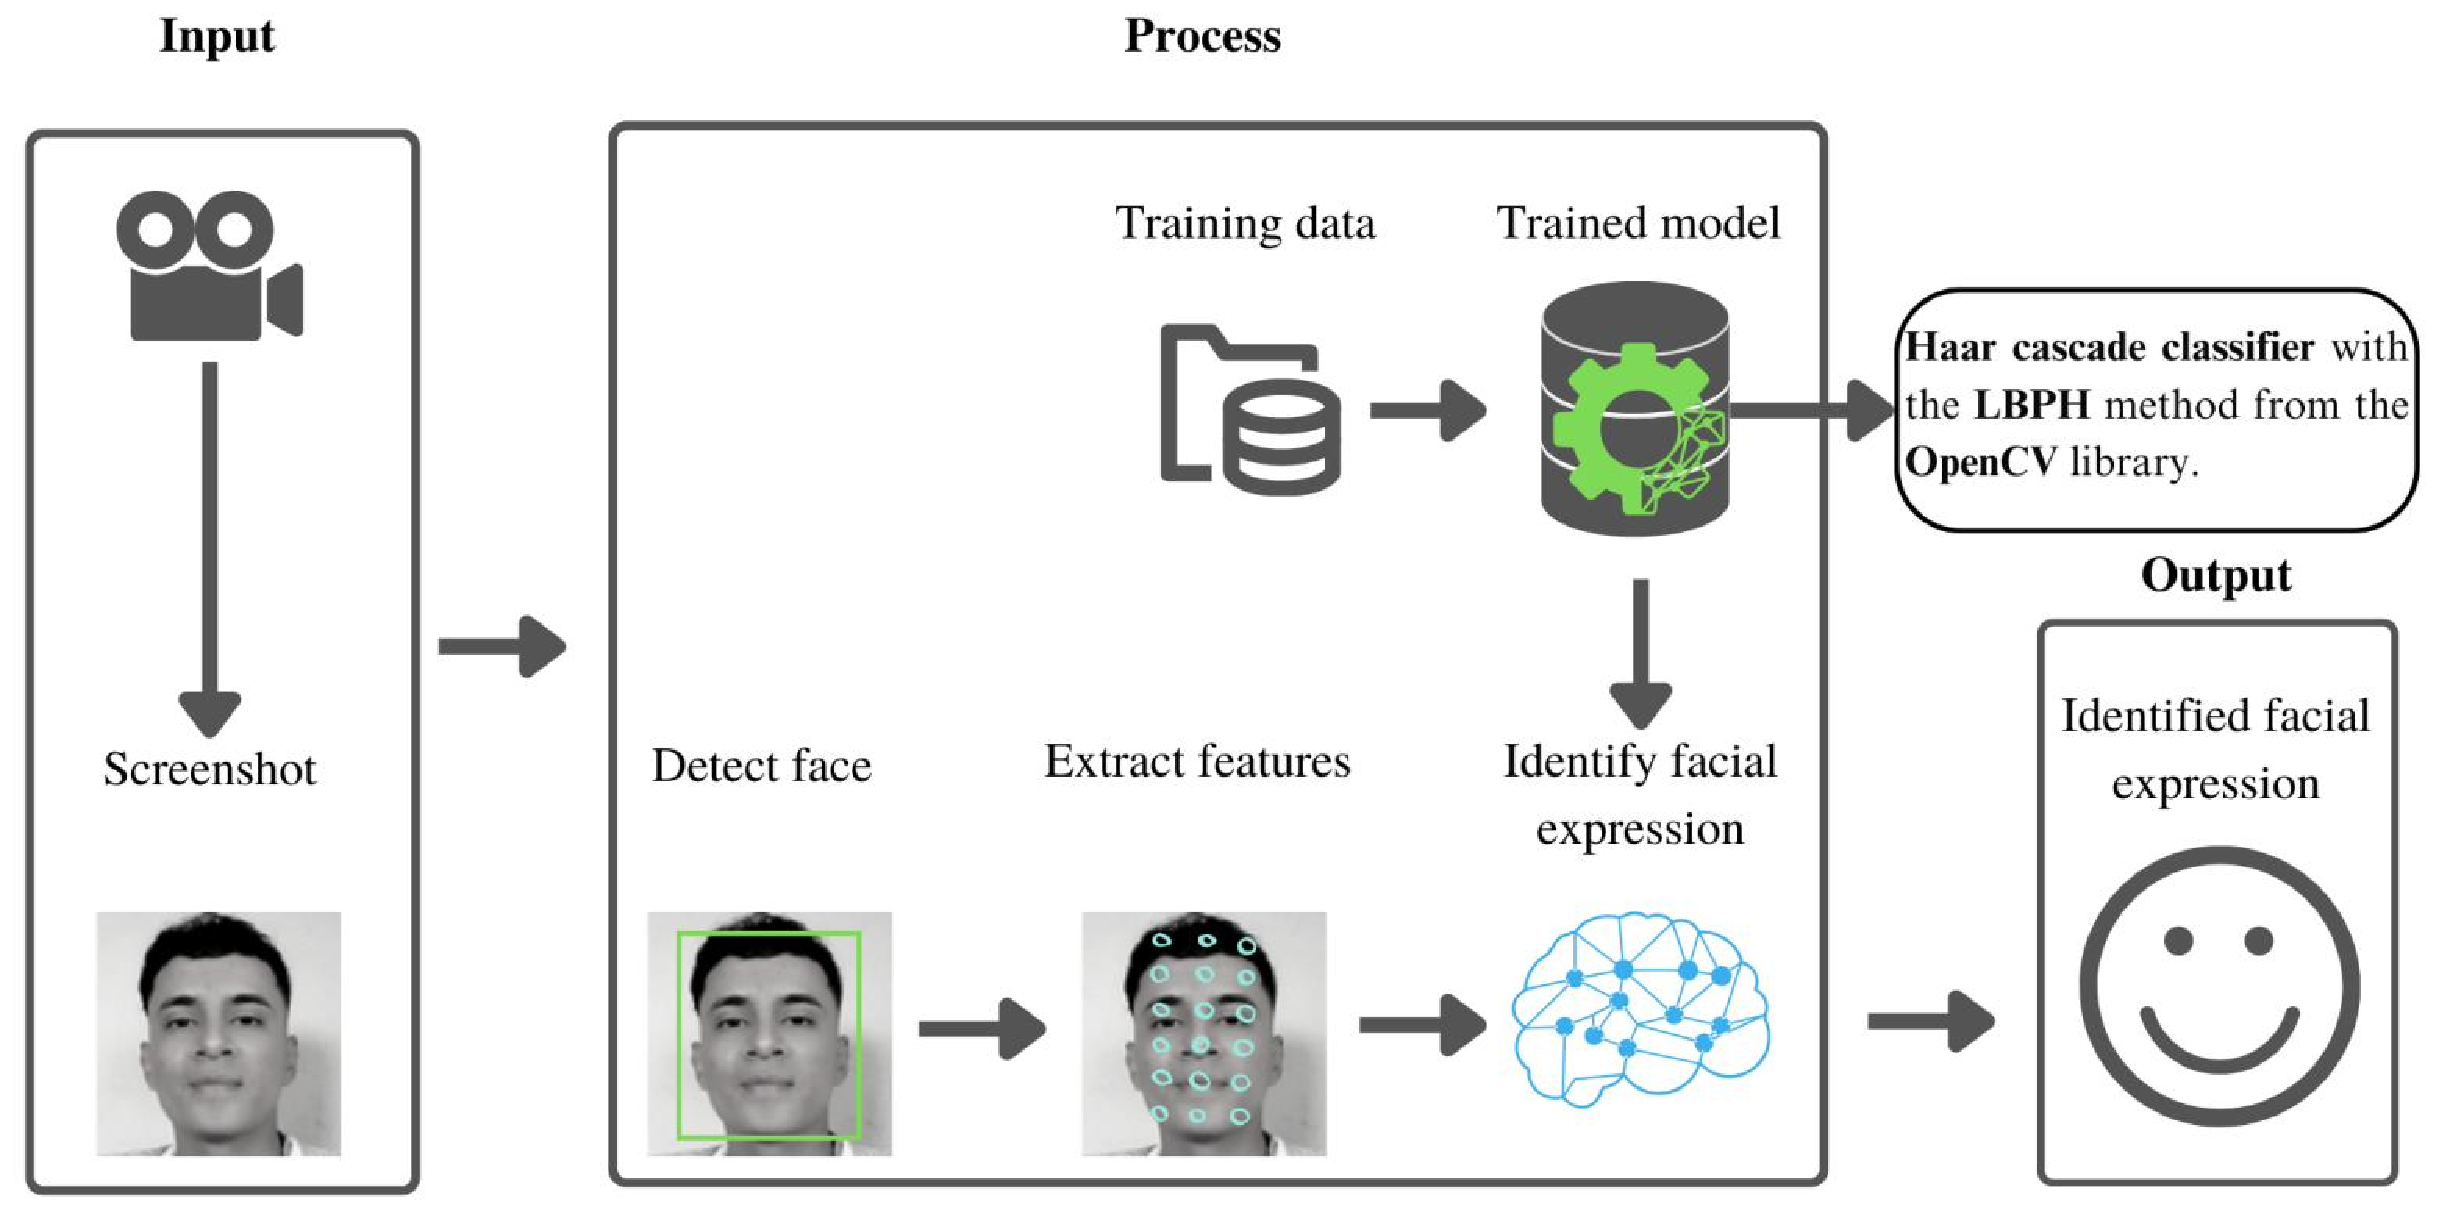
\includegraphics[frame,scale=0.5, width=\linewidth]{figs/Figure_3}
                    \caption{Facial expression recognition procedure used in the Torddis system.\label{fig:FacialExpression}}
                \end{figure}
                
                \paragraph{Drowsiness Detection Methods.}
                Drowsiness detection methods require an input image containing a human face. These methods perform image preprocessing to extract characteristic eye landmarks and then analyze whether the subject's eyes are closed. Table~\ref{tab:sleep-detection-methods} summarizes the methods used for drowsiness detection.
                
                \begin{table}[!htbp]
                    \centering
                    \caption{Drowsiness detection methods.}
                    \label{tab:sleep-detection-methods}
                    \begin{tabular}{p{0.20\textwidth}p{0.58\textwidth}p{0.10\textwidth}}
                        \toprule
                        \textbf{Algorithm} & \textbf{Purpose} & \textbf{Accuracy} \\
                        \midrule
                        
                        MediaPipe Face Mesh & Detection of facial landmarks with 468 3D points \citep{Shanmugam2022Comparative}. & \multicolumn{1}{r}{99.87\%} \\
                        
                        SVM & Eye tracking \citep{Altameem2021Early}. & \multicolumn{1}{r}{83.25\%} \\
                        
                        Viola-Jones & Drowsiness detection \citep{Teja2021Real}. & \multicolumn{1}{r}{92.00\%} \\
                        
                        CNN & Trained on four gestures: eyes open, eyes closed, yawning, and not yawning \citep{I2022Raspberry}. & \multicolumn{1}{r}{80.00\%} \\
                        \bottomrule
                    \end{tabular}
                \end{table}
                
                The SVM \citep{Altameem2021Early}, CNN \citep{I2022Raspberry}, and Viola-Jones \citep{Teja2021Real} algorithms were discarded due to their limitations in accuracy for drowsiness detection and their complexity in real-time implementation. Specifically, SVM and Viola-Jones require intensive preprocessing and struggle to handle variations in lighting and posture, whereas CNNs, although accurate, demand high computational capacity for inference on low-power devices.
                
                For these reasons, the selected algorithm was MediaPipe Face Mesh \citep{Shanmugam2022Comparative}, as it offers an optimal balance between accuracy and computational efficiency, enabling real-time drowsiness detection with low latency and without the need for specialized hardware.
                
                \paragraph{Object Recognition Methods}
                Computer vision enables the automatic detection of the structure and properties of a potential dynamic three-dimensional world. First, an input image containing one or more objects is required. Then, image preprocessing is performed to extract features from the segmented image. Table~\ref{tab:object-recognition} describes a list of object recognition algorithms.
                
                \begin{table}[!htbp]
                    \caption{Algorithms for object recognition.}
                    \label{tab:object-recognition}
                    \centering
                    \begin{tabular}{
                            >{\raggedright\arraybackslash}p{0.15\textwidth}
                            >{\raggedright\arraybackslash}p{0.24\textwidth}
                            >{\raggedright\arraybackslash}p{0.35\textwidth}
                            >{\raggedright\arraybackslash}p{0.15\textwidth}
                        }
                        \toprule
                        \textbf{Algorithm} & \textbf{Technology and Implementation} & \textbf{Purpose} & \textbf{Accuracy} \\
                        \midrule
                        
                        CNN & Python, TensorFlow, Keras, CIFAR-10 (25 training epochs) & Image classification and recognition, specifically of airplanes \citep{Sudharshan2018Object}. & 96.00\% \\
                        
                        Viola Jones & Haar-like features, AdaBoost, Cascade Classifier & Face detection and eye tracking (blinking detection, eye position) \citep{Teja2021Real} & 
                        Face: 98\%
                        Eyes: 94\%
                        With glasses: 82\%
                        Without glasses: 92\%\\
                        
                        PERCLOS\textsuperscript{a} & EAR\textsuperscript{b} computed from IR\textsuperscript{c} images, blink monitoring & Determine driver drowsiness level through eyelid closure percentage \citep{Teja2021Real} & Not applicable (dependent on EAR) \\
                        
                        YOLOv4 + CNN-29 & Python, OpenCV, Darknet YOLOv4 & Automatic detection of faults in solar panels (defective cells, hotspots, electrical failures) using thermal images captured by drone \citep{Zou2022Drone} & Solar panel: 100\% (confidence);
                        Defective cells: 32\% initially, up to 89\% after retraining \\
                        
                        YOLO & CNN (YOLO), bounding boxes and IOU\textsuperscript{d} score & Object detection in the environment (e.g., bottles) to trigger alerts \citep{Teja2021Real}. & 98.00\% \\
                        
                        \multirow[t]{3}{*}{YOLOv4} & \multirow[t]{2}{*}{\parbox[t]{\linewidth}{Implemented with Darknet and optimized with TensorRT\textsuperscript{e} on Jetson Nano platform}} & Real-time detection of Vietnamese vehicles \citep{Minh2021Performance}. & 90.00\% \\
                        
                        & & Real-time detection of Vietnamese license plates \citep{Minh2021Performance}. & 92.00\% \\
                        
                        & Implemented on a digital chip with custom CNN architecture. Uses 2D\textsuperscript{f} Winograd Convolution with MSAM\textsuperscript{g}. Trained with PASCAL VOC 2007/2012\textsuperscript{h} in PyTorch & Detection of objects and people \citep{Liu2021Objects}. & mAP\textsuperscript{i}: 73.01\% \\
                        
                        \multirow[t]{2}{*}{\parbox[t]{\linewidth}{MobileNetV2-SSD}} & \multirow[t]{2}{*}{\parbox[t]{\linewidth}{Implemented with PyTorch and accelerated with TensorRT}} & Real-time detection of Vietnamese vehicles \citep{Minh2021Performance}. & 85.00\% \\
                        
                        & & Real-time detection of Vietnamese license plates \citep{Minh2021Performance}. & 90.00\% \\
                        \bottomrule
                    \end{tabular}
                    %\vspace{0mm}
                    %\raggedright
                    \begin{flushleft}
                        \textsuperscript{a} PERcentage of eye CLOSure: metric used in drowsiness detection systems. \textsuperscript{b} Eye Aspect Ratio: metric relating eye height and width to estimate openness. \textsuperscript{c} Infrared: type of image captured via IR sensors. \textsuperscript{d} Intersection over Union: metric measuring overlap between predicted and actual bounding boxes in object detection tasks. \textsuperscript{e} TensorRT: NVIDIA inference optimization library that accelerates deep learning models for efficient execution on GPU (Graphics Processing Unit). \textsuperscript{f} 2D: bidimensional, two-dimensional matrices in images. \textsuperscript{g} MSAM (Modified Spatial Attention Module): spatial attention module that enhances the network's focus on relevant image regions. \textsuperscript{h} PASCAL VOC 2007/2012: benchmark datasets for object detection (people, vehicles, animals). \textsuperscript{i} mean Average Precision.
                    \end{flushleft}
                \end{table}
                
                Based on the information presented in Table~\ref{tab:object-recognition}, the selected algorithm was \textit{Sequential} from the \textit{TensorFlow} library in combination with \textit{Keras} due to its accuracy, optimal performance, ease of training, and widespread use for real-time object recognition. MobileNetV2 combined with SSD was discarded due to its lower object recognition accuracy compared to other models. YOLO was also discarded because of the high GPU (Graphics Processing Unit) requirements for proper operation.
                
                \paragraph{Object Recognition Procedure}
                This method consists of the following steps:
                
                \begin{enumerate}
                    \item A photograph is taken to capture the objects on the desk or in the area where the child is working.
                    
                    \item The image is preprocessed and segmented into parts corresponding to potential objects.
                    
                    \item Feature extraction is performed on the segmented image.
                    
                    \item Finally, the extracted features are compared with a computational model previously trained on a dataset containing the objects to be recognized.
                \end{enumerate}
                
                Computer vision enables the automatic detection of the structure and properties of a potential dynamic three-dimensional world based on one or more two-dimensional images of the scene \citep{Cruz2013}. Figure~\ref{fig:ObjectRecognition} illustrates the object recognition procedure used in the Torddis system implementation.
                
                \begin{figure}[!htbp]
                    \centering
                    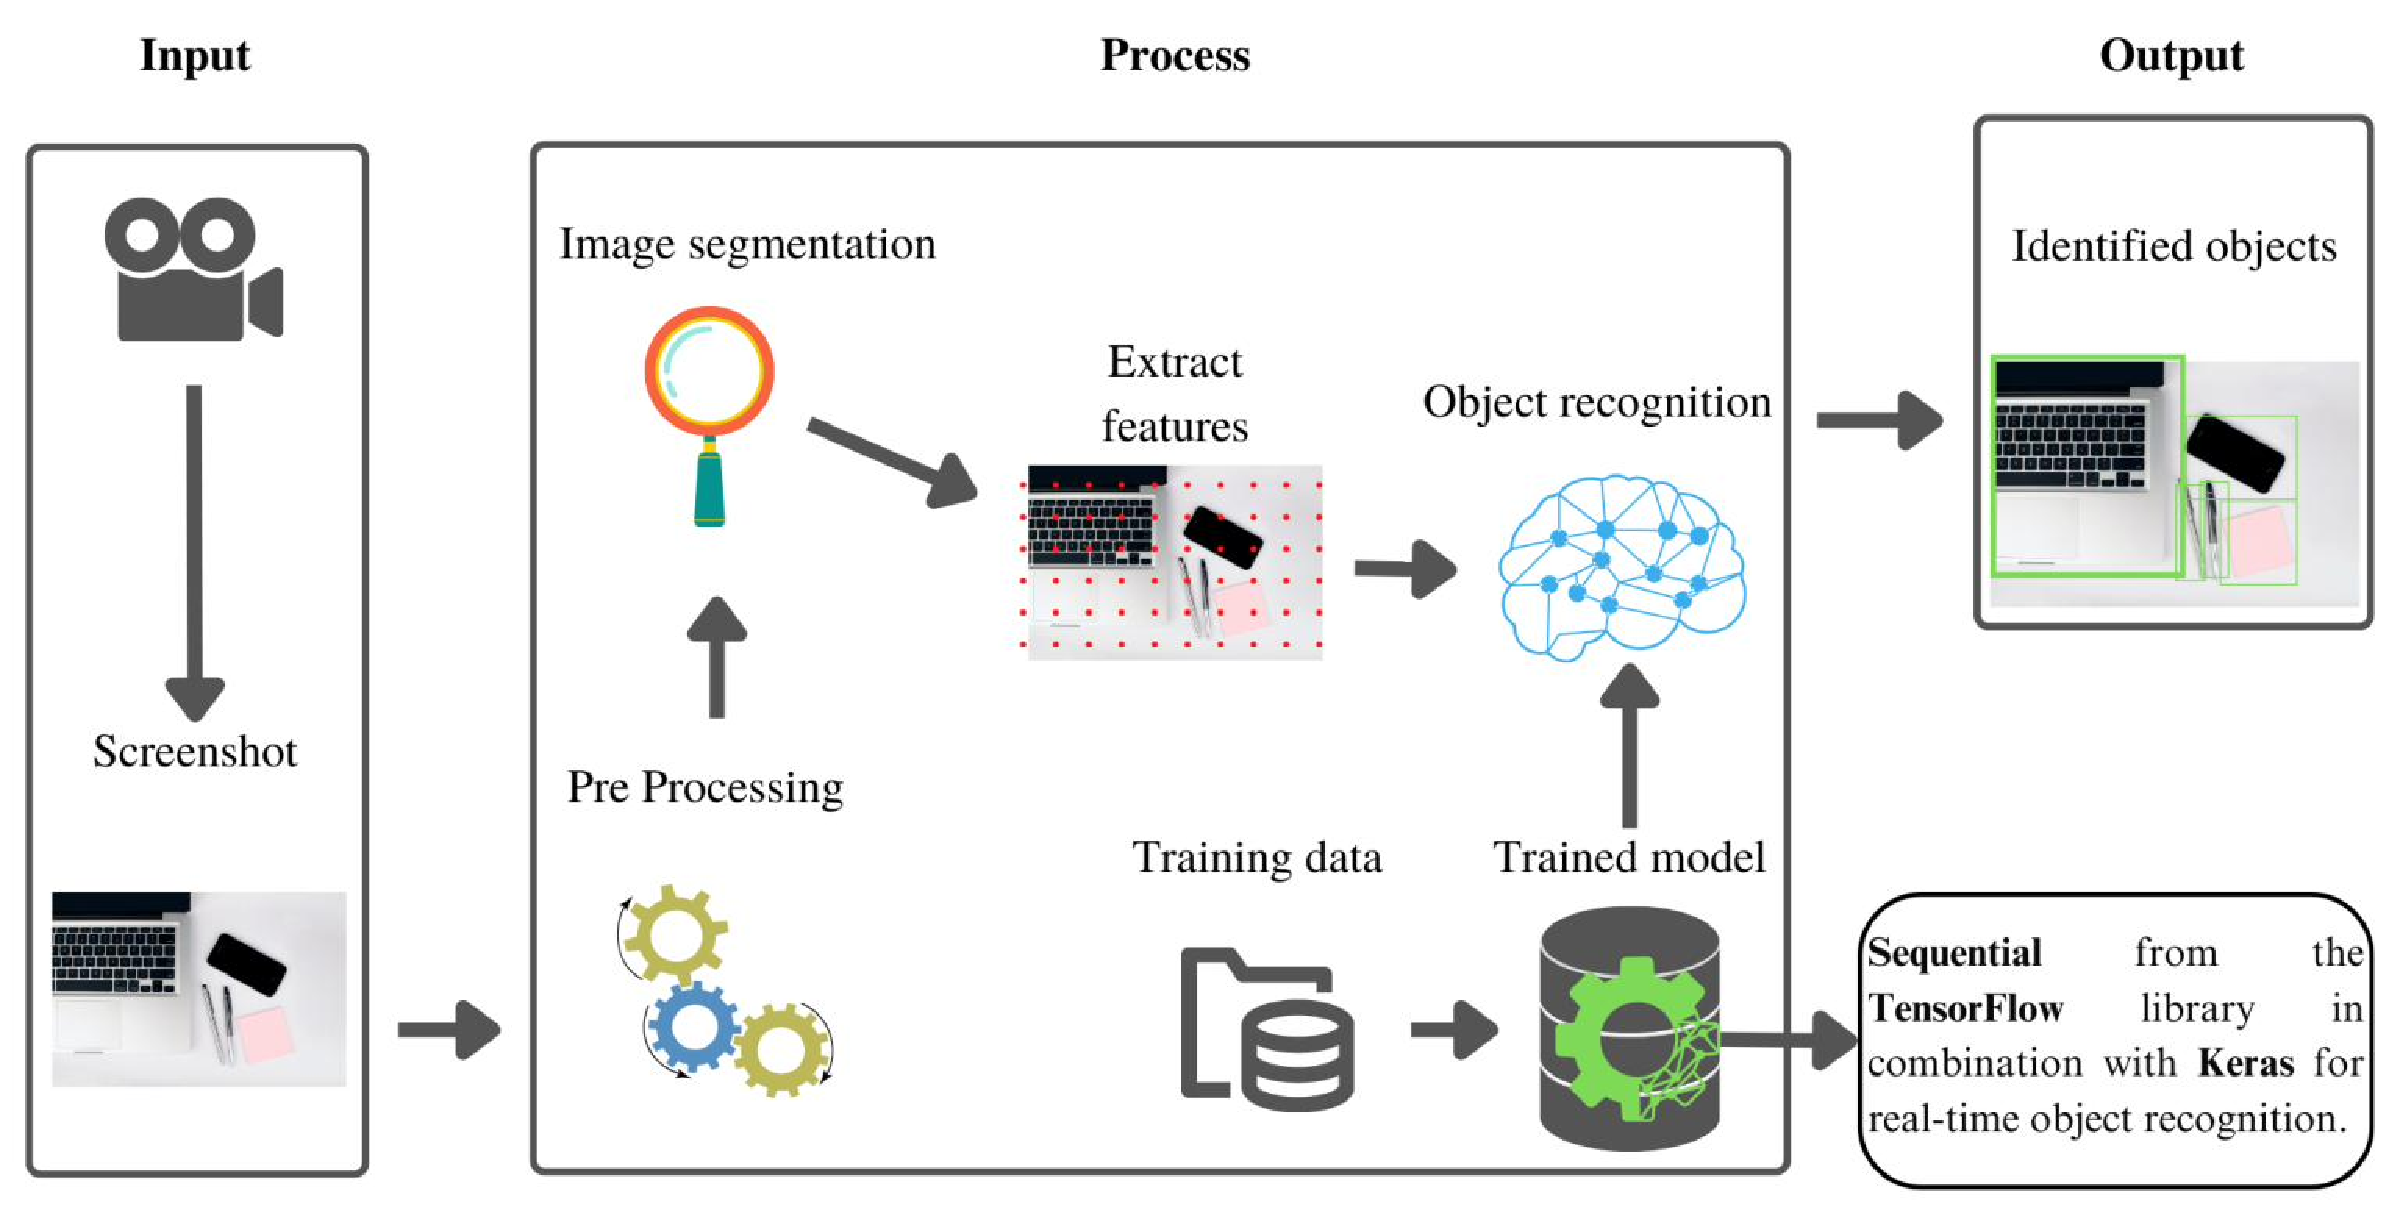
\includegraphics[frame,scale=0.5, width=\linewidth]{figs/Figure_4}
                    \caption{Object recognition procedure used in the Torddis system.\label{fig:ObjectRecognition}}
                \end{figure}
                
                The analysis highlights that Torddis outperforms existing market solutions due to its integration of facial and object recognition technologies to effectively monitor distractions. This advantage is reflected in the high acceptance rates among tutors and the positive results observed in students, positioning the system as a superior solution for monitoring and supporting academic tasks at home \citep{Deng2024Does}.
                Following the elicitation of system requirements, the architecture of the Torddis system was initially designed (see Figure~\ref{fig:TorddisArchitecture}). Subsequently, with the assistance of the TDDT4IoTS tool \citep{Guerrero2024Test}, the IoT device of the system was designed.
                                
                \begin{figure}[!htbp]
                    \centering
                    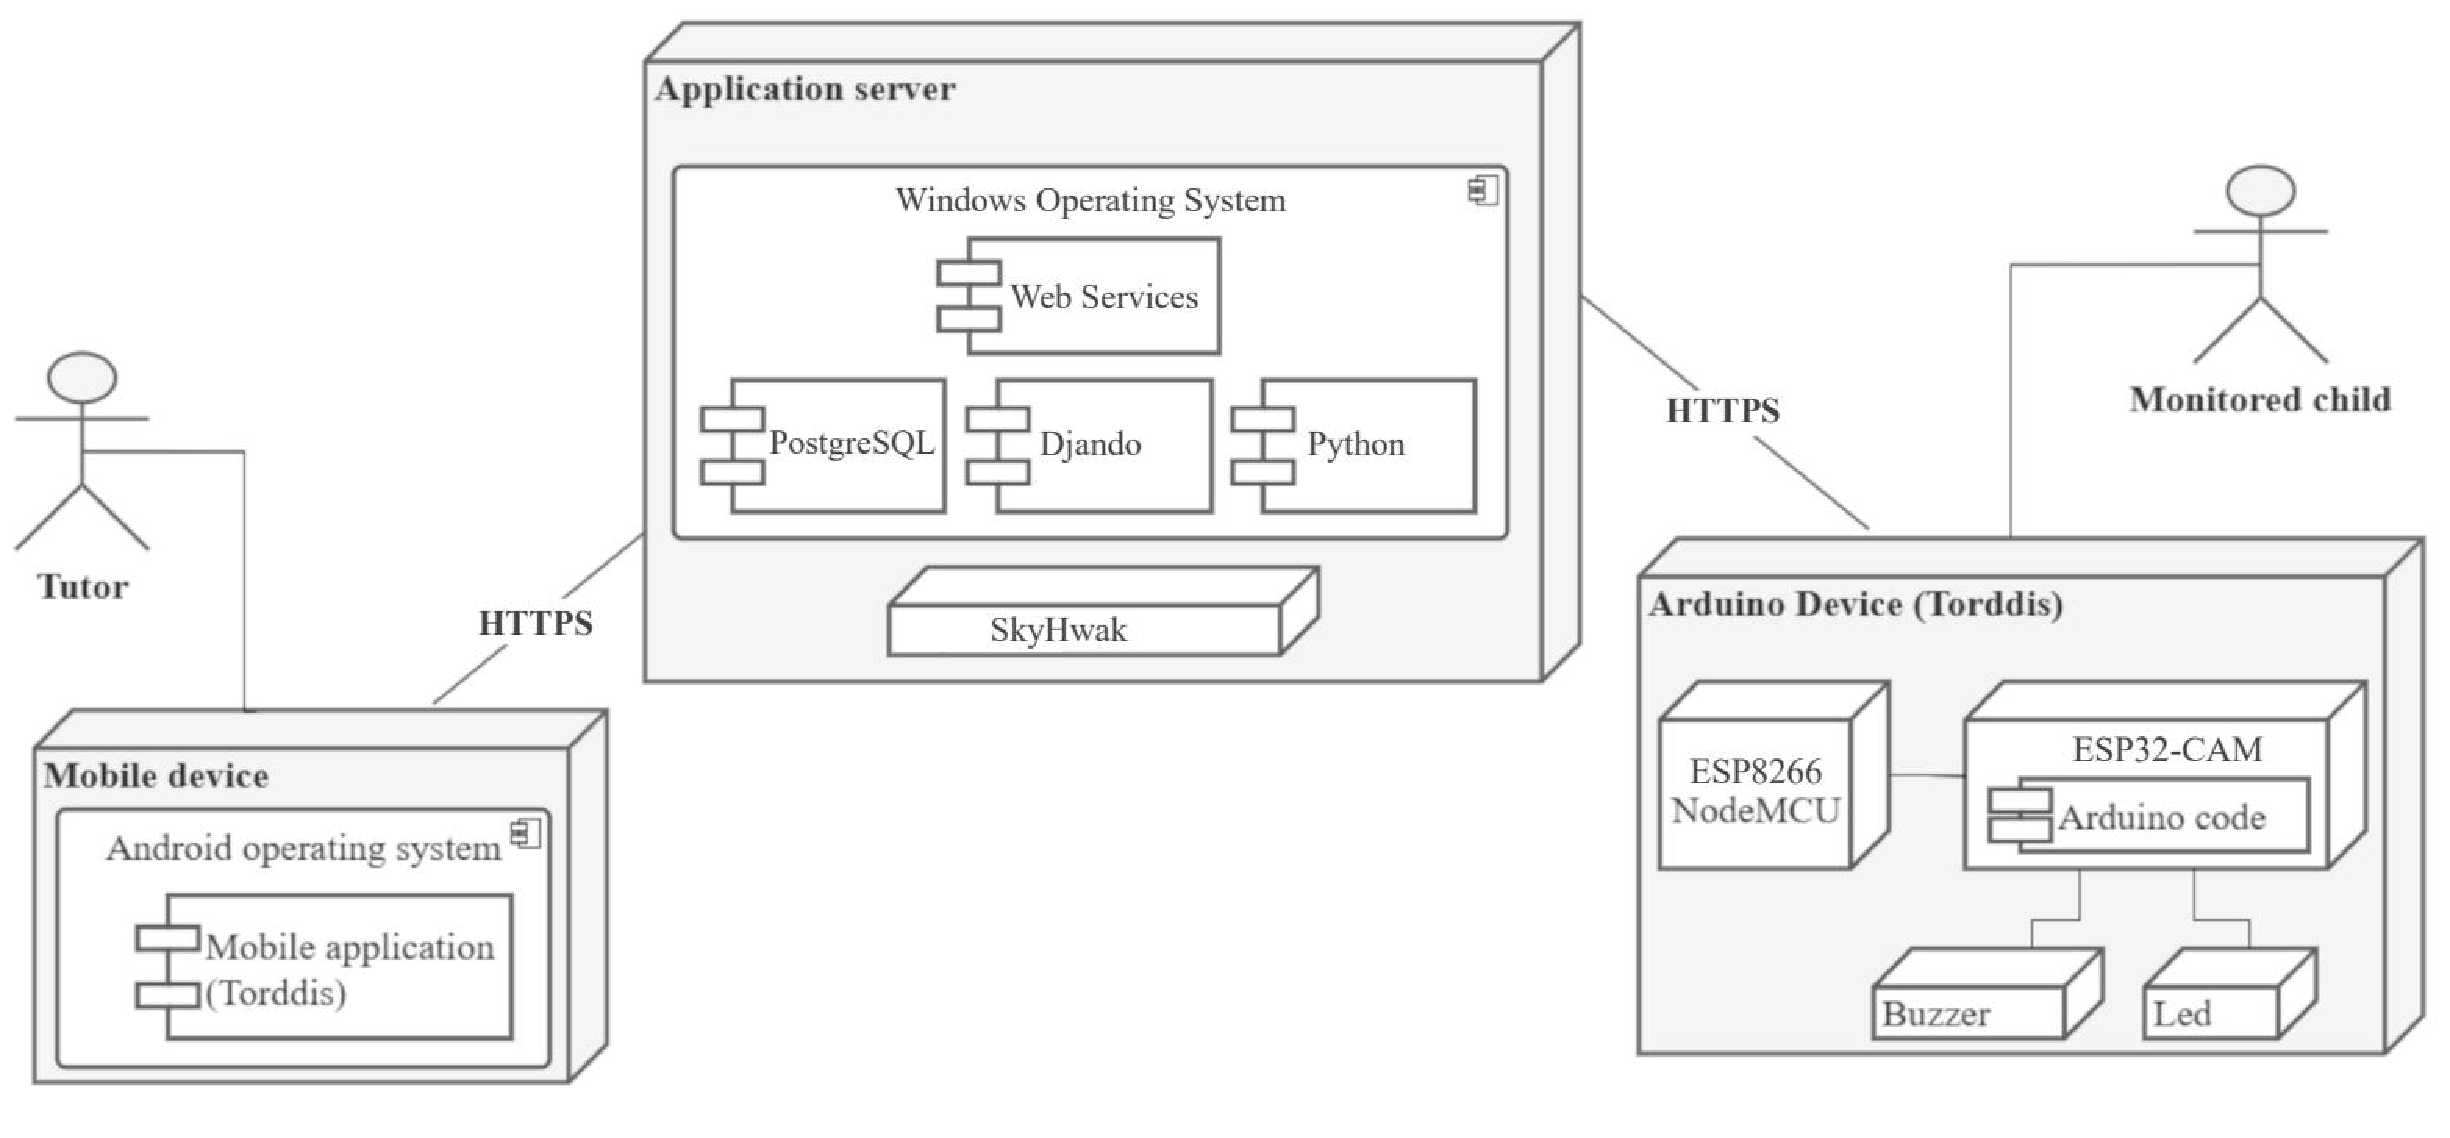
\includegraphics[frame,scale=0.5, width=0.9\linewidth]{figs/Figure_5}
                    \caption{Deployment diagram (nodes) of the Torddis system.\label{fig:TorddisArchitecture}}
                \end{figure}
                
                Figure~\ref{fig:TorddisDevice} illustrates the structural design of the IoT device, highlighting the components used in its construction, which are:
                
                \begin{figure}[!htbp]
                    \centering
                    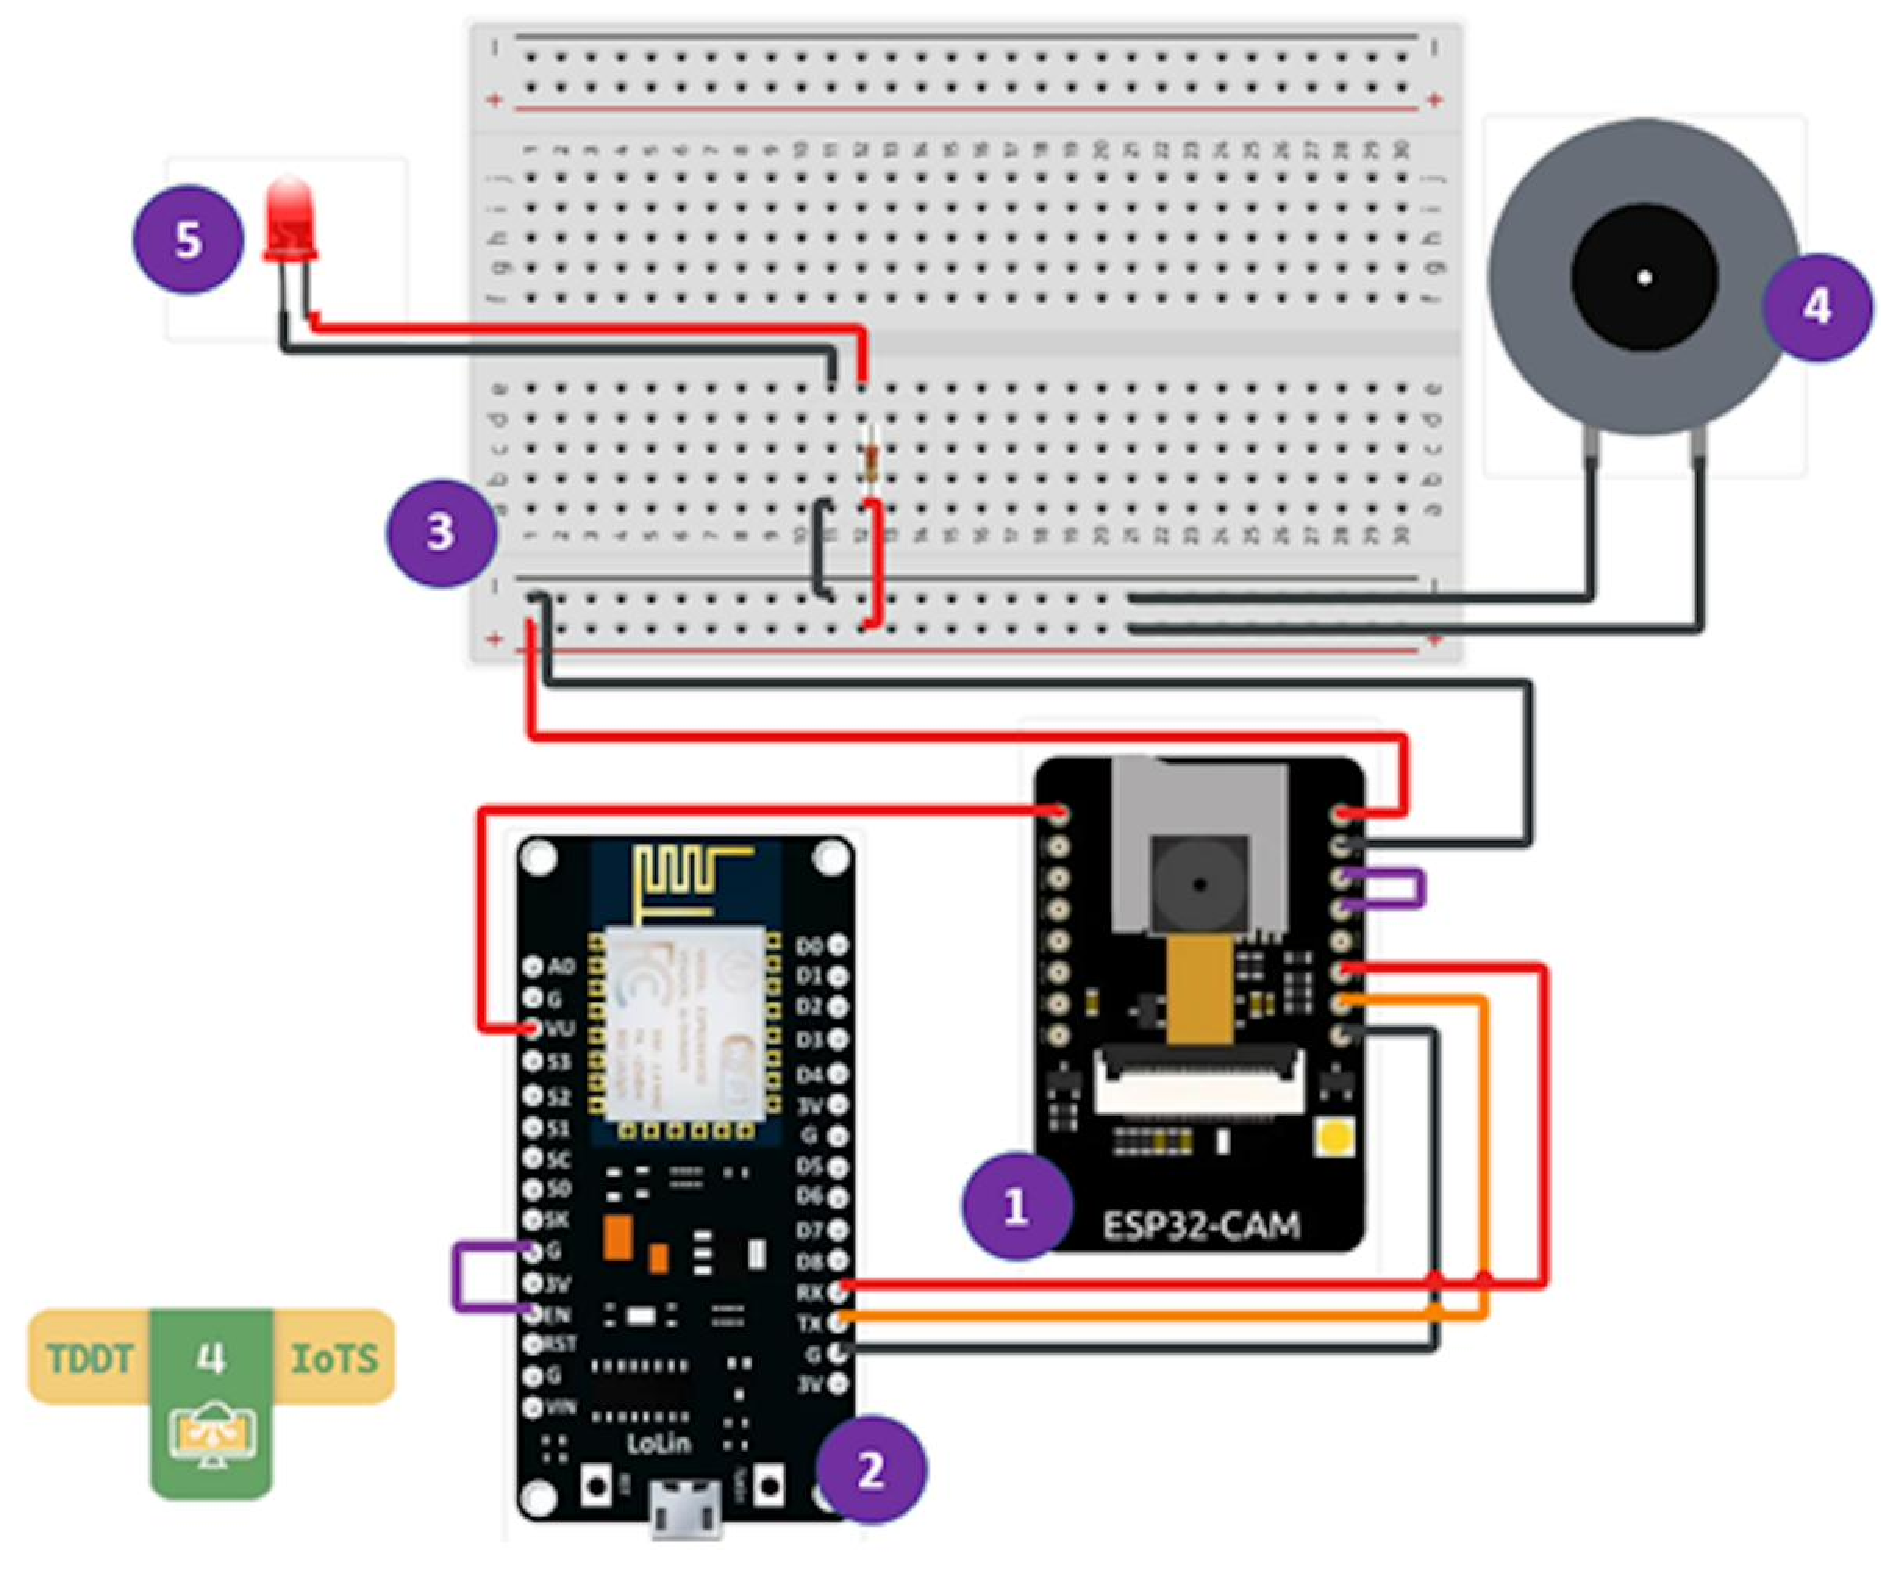
\includegraphics[frame,scale=0.5, width=0.78\linewidth]{figs/Figure_6}
                    \caption{Design of the IoT device of the Torddis system.\label{fig:TorddisDevice}}
                \end{figure}
                
                \begin{enumerate}
                    \item ESP32-CAM board
                    \item ESP8266 NodeMCU board
                    \item Protoboard
                    \item Passive buzzer
                    \item Red LED
                \end{enumerate}
                With the system architecture and coarse-grained functionalities already defined, the fine-grained requirements were elicited to ensure a successful implementation of Torddis. Figure~\ref{fig:Fine-GrainedUseCase} presents the use case diagram that clearly and specifically represents the problem domain.
                
                \begin{figure}[!htbp]
                    \centering
                    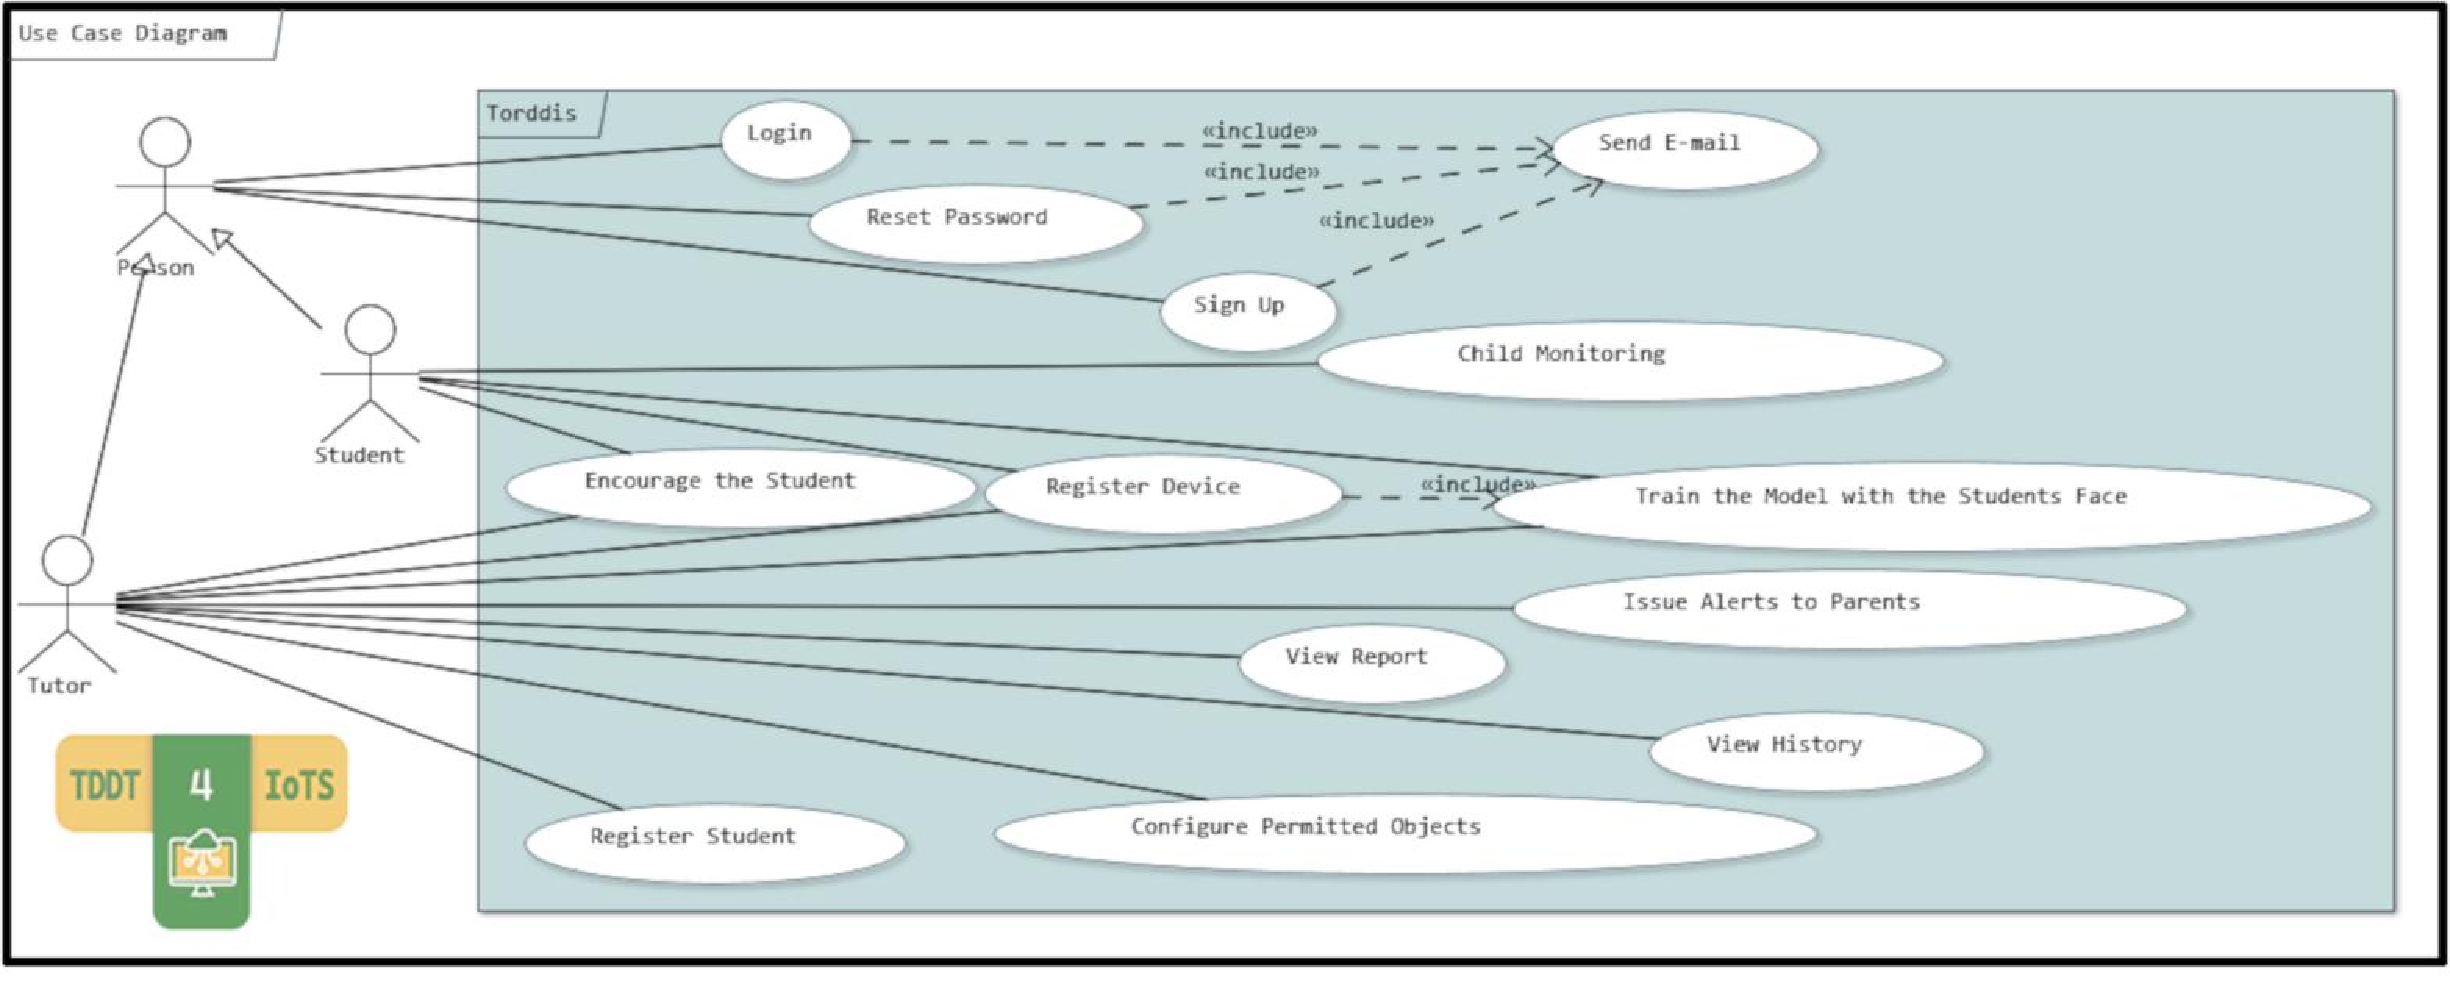
\includegraphics[scale=1, width=\linewidth]{figs/Figure_7}
                    \caption{Fine-grained use case diagram of the Torddis system.\label{fig:Fine-GrainedUseCase}}
                \end{figure}
                
                Table~\ref{tab:use-case-register-device} presents one of the fine-grained use cases in an extended format so that developers can implement the corresponding business logic and ensure the system meets the established specifications.
                
                \begin{table}[!htbp]
                    \centering
                    \caption{Use Case: Register Torddis device}
                    \label{tab:use-case-register-device}
                    \begin{tabularx}{\textwidth}{|l|X|}
                        \hline
                        \textbf{Use Case} & Register Torddis device \\ \hline
                        \textbf{Description} & The tutor enters the MAC address of the Torddis device. The system registers the device in the database and displays a confirmation message. \\ \hline
                        \textbf{Actors} & Tutor \\ \hline
                        \textbf{Preconditions} & User is authenticated as a tutor. \\ \hline
                        \textbf{Postconditions} & The tutor's Torddis device is linked. \\ \hline
                        \textbf{Main Flow} &
                        \begin{enumerate}
                            \item The use case begins when the tutor accesses the device-linking interface.
                            \item The system displays a form with the controls to link the device: MAC address input.
                            \item The tutor enters the MAC address and selects the save option (see Alt 1).
                            \item The system stores the data in the database (see E1).
                            \item The system provides feedback indicating a successful operation.
                            \item The use case ends when the system displays the facial training interface.
                        \end{enumerate} \\ \hline
                        \textbf{Alternative Flows} &
                        \textbf{Alt 1.} The tutor does not wish to register the Torddis device:
                        \begin{enumerate}
                            \item[3.] The use case ends when the tutor cancels the operation.
                        \end{enumerate} \\ \hline
                        \textbf{Exceptions} &
                        \textbf{E1.} Error when registering the Torddis device:
                        \begin{enumerate}
                            \item[4.] The system displays a message: \textit{Error registering the Torddis device. Please try again.}
                            \item[5.] The tutor resumes from step 3 of the main flow.
                        \end{enumerate} \\ \hline
                    \end{tabularx}
                \end{table}
                
                Acknowledging technical limitations—such as object detection error rates and resource consumption—has made it possible to identify concrete areas for improvement. The implementation of lighter and optimized models, together with real-time calibration mechanisms, will ensure greater accuracy and performance of the system, even in less favorable environments \citep{Falzetti2024Promoting}.
                Among the system modeling tools employed, structural models were used—such as class diagrams (see Figure~\ref{fig:ClassDiagram})—which were generated directly by the TDDT4IoTS tool \citep{Guerrero2024Test} based on the use cases that specify the system to be developed.
                
                \begin{figure}[!htbp]
                    \centering
                    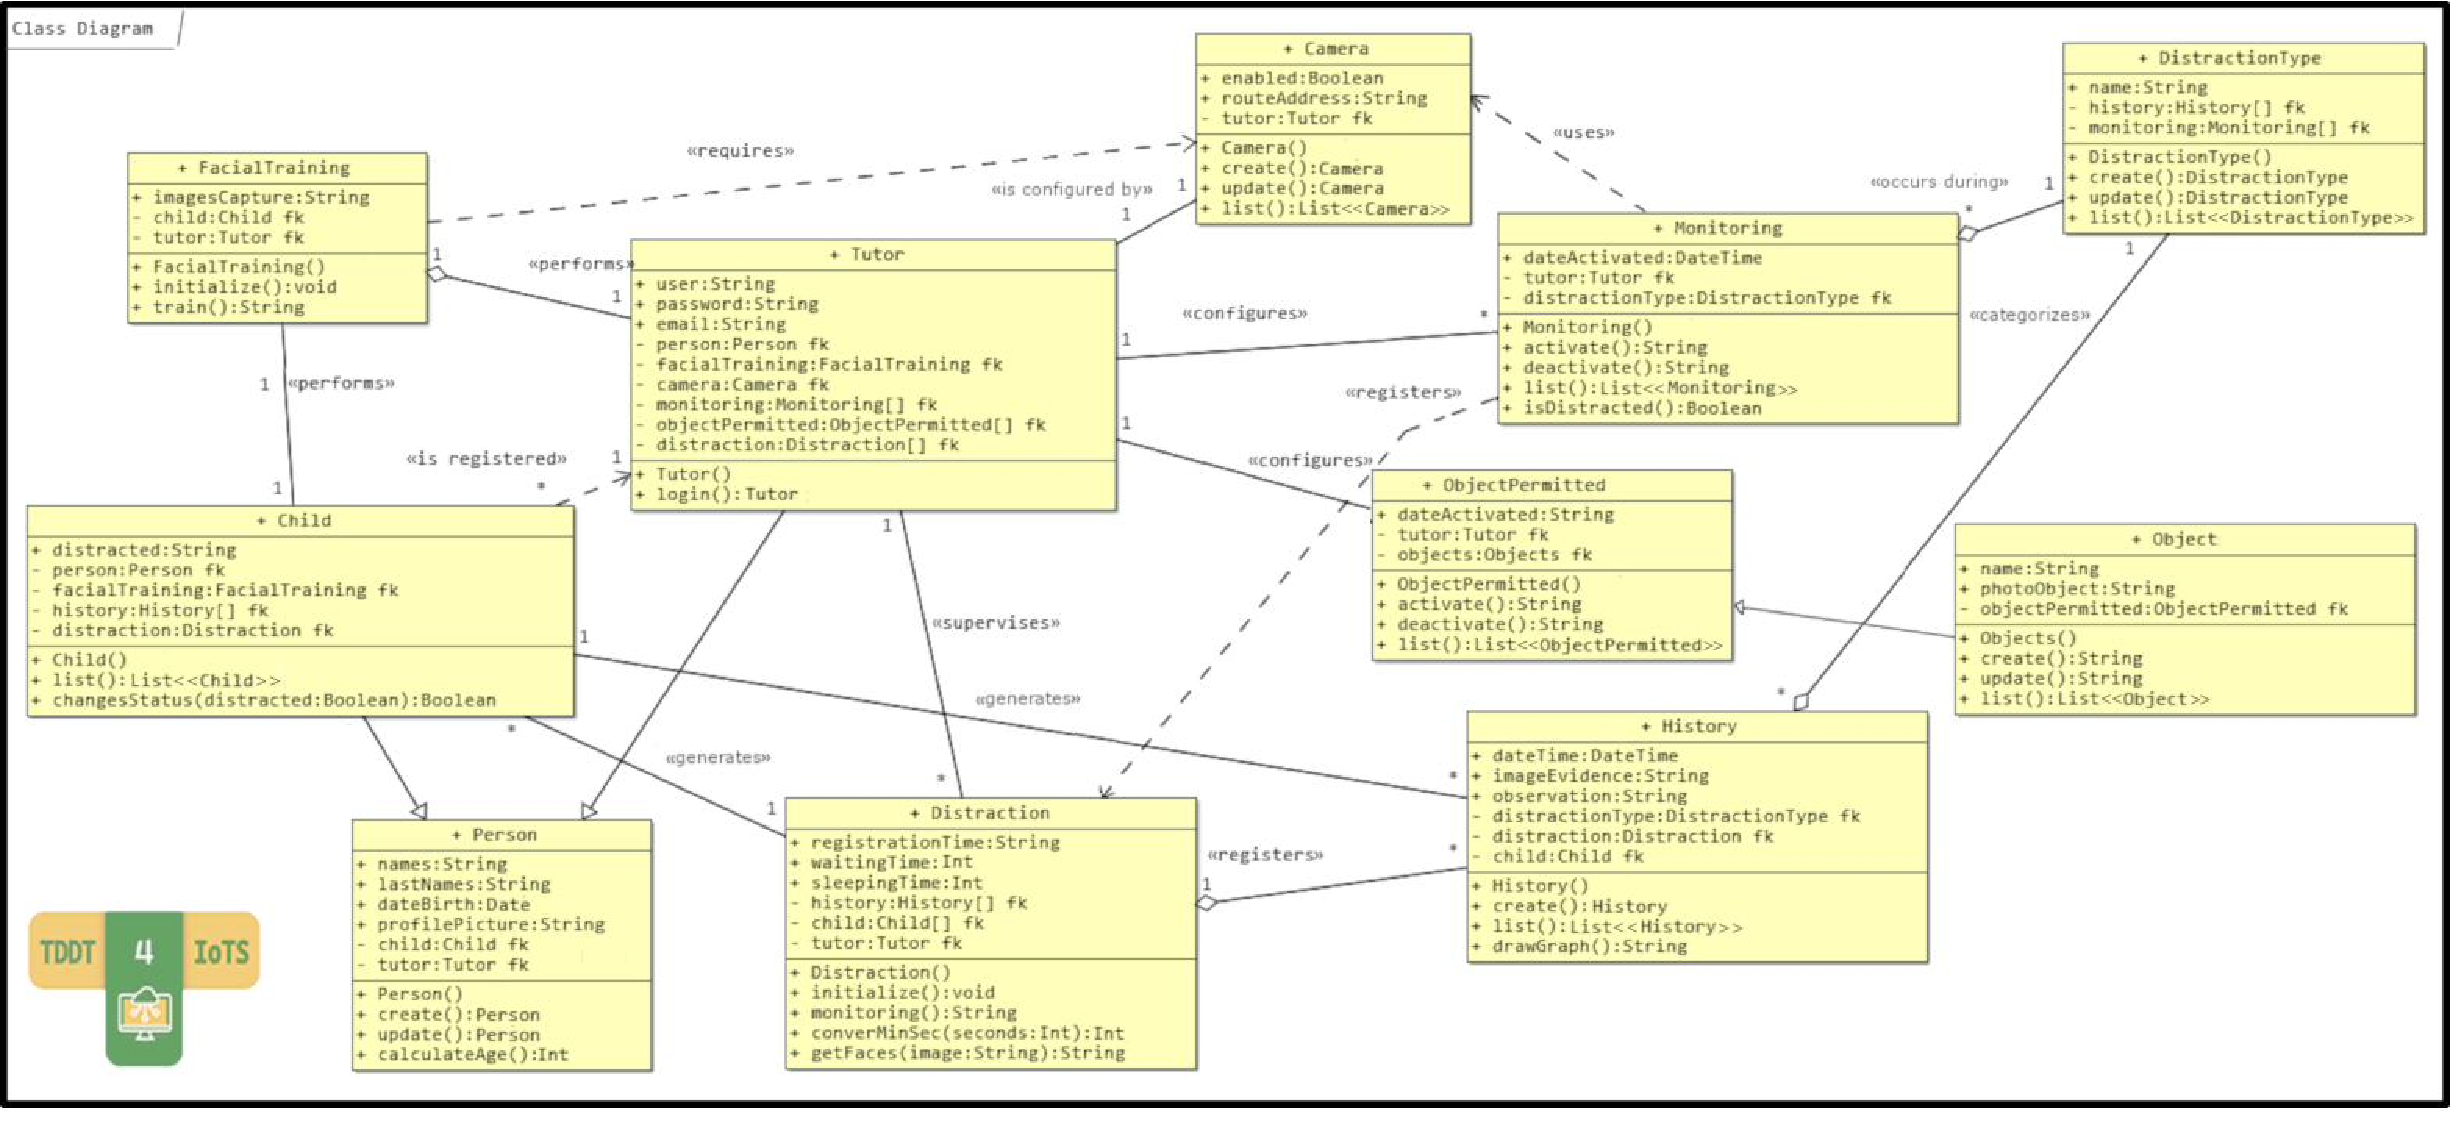
\includegraphics[frame,scale=0.5, width=\linewidth]{figs/Figure_8}
                    \caption{Class diagram of the Torddis system.\label{fig:ClassDiagram}}
                \end{figure}
                
                In addition, the AI computational models for monitoring learner events based on specified distraction parameters were obtained and refined by adjusting configurations such as the number of hidden layers and the number of training epochs.
                The unit and integration tests that can be written in code (such as those related to database connections, web service testing, among others) were also automatically generated by the TDDT4IoTS tool \citep{Guerrero2024Test}. The data for unit testing (e.g., mobile application functions such as alert playback and drowsiness detection) were mainly obtained during the detailed requirements analysis phase, whereas the integration tests were derived during the system architecture design phase (i.e., communication between the ESP8286 NodeMCU and web services). Some of these integration tests were manually written and executed, such as the interface with the web services.
                
                Figure~\ref{fig:stages-tests} illustrates the relationship between the test data acquisition and the system life cycle phases. All system and acceptance tests were manually written and executed. 
                                
                \begin{figure}[!htbp]
                    \centering
                    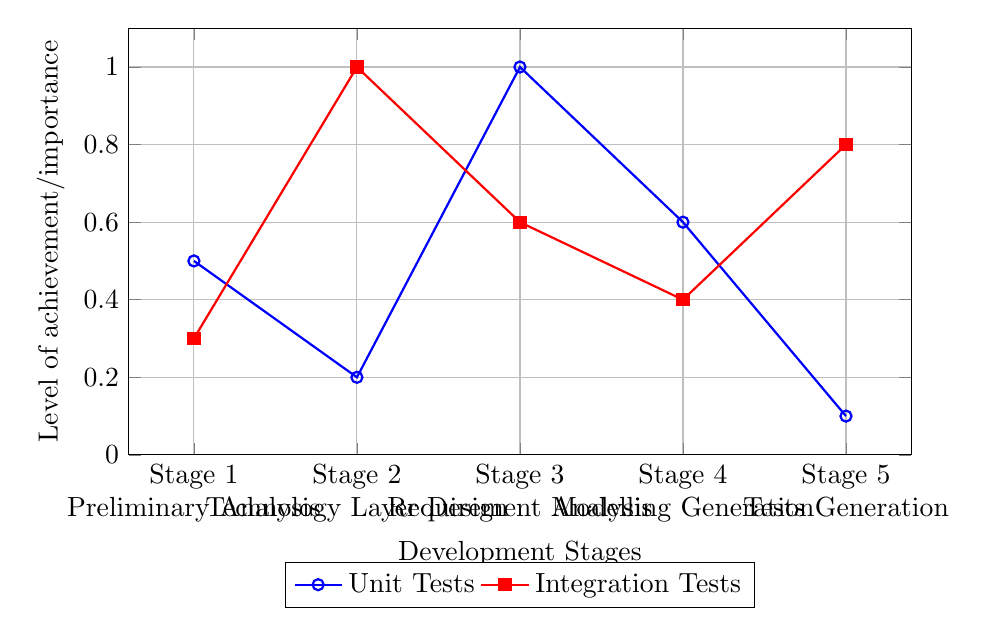
\begin{tikzpicture}
                        \begin{axis}[
                            width=0.95\linewidth,
                            height=7cm,
                            xlabel={Development Stages},
                            ylabel={Level of achievement/importance},
                            ymin=0, ymax=1.1,
                            xtick={1,2,3,4,5},
                            xticklabels={
                                \shortstack{Stage 1\\Preliminary Analysis},
                                \shortstack{Stage 2\\Technology Layer Design},
                                \shortstack{Stage 3\\Requirement Analysis},
                                \shortstack{Stage 4\\Modelling Generation},
                                \shortstack{Stage 5\\Tests Generation}
                            },
                            ytick={0,0.2,0.4,0.6,0.8,1.0},
                            legend style={at={(0.5,-0.25)}, anchor=north, legend columns=-1},
                            grid=major
                            ]
                            
                            \addplot[
                            color=blue,
                            mark=o,
                            thick
                            ]
                            coordinates {(1,0.5) (2,0.2) (3,1.0) (4,0.6) (5,0.1)};
                            \addlegendentry{Unit Tests}
                            
                            \addplot[
                            color=red,
                            mark=square*,
                            thick
                            ]
                            coordinates {(1,0.3) (2,1.0) (3,0.6) (4,0.4) (5,0.8)};
                            \addlegendentry{Integration Tests}
                            
                        \end{axis}
                    \end{tikzpicture}
                    \caption{Relationship between test data Acquisition and the Torddis life cycle phases.}
                    \label{fig:stages-tests}
                \end{figure}
                
                Tables~\ref{tab:create-tutor-account-test-case}, \ref{tab:login-test-case}, \ref{tab:face-training-test-case}, \ref{tab:device-registration-test-case}, and \ref{tab:configure-object-usage-test-case} summarize system test cases that were also used as acceptance tests, enabling verification that Torddis satisfies the defined requirements. These tests were authored and executed during the project—including validation with tutor users—to ensure alignment with the specifications.
                
                Table~\ref{tab:create-tutor-account-test-case} introduces the test case for tutor account creation, which serves as the system’s entry point. It is part of the documented system and acceptance test suite. The objective is to ensure that tutor registration is correctly recorded in accordance with the specifications \citep{Sciarra2024Smash}.
                
                \begin{table}[!htbp]
                    \centering
                    \caption{Test case for tutor account creation.}
                    \label{tab:create-tutor-account-test-case}
                    \begin{tabularx}{\textwidth}{l X}
                        \toprule
                        \textbf{Test Case ID:} & PU-1 \\
                        \textbf{Test Case Name:} & Tutor Account Creation \\
                        \textbf{Expected Outcome:} & Successfully create a tutor account \\
                        \midrule
                        \multicolumn{2}{c}{\textbf{Test Case Procedure}} \\
                        \midrule
                        \multicolumn{1}{c}{\textbf{Step No.}} & \textbf{Step Description} \\
                        \midrule
                        \multicolumn{1}{c}{1} & Open the mobile application. \\
                        \multicolumn{1}{c}{2} & Select the ``Sign Up'' option. \\
                        \multicolumn{1}{c}{3} & Enter the registration data.
                        \begin{itemize}
                            \item First name: Carlos Iván
                            \item Last name: Almeida Dueñas
                            \item Email: carlos.almeida2017@utec.edu.ec
                            \item Date of birth: 10/01/2000
                            \item Username: calmeidad
                            \item Password: XXXXXX
                        \end{itemize}\\
                        \multicolumn{1}{c}{4} & Select the ``Create Account'' option. \\
                        \bottomrule
                    \end{tabularx}
                \end{table}
                
                Table~\ref{tab:login-test-case} describes the test case that verifies signing in with a tutor account, explicitly included among the acceptance tests. It is also aligned with the non-functional requirement mandating encryption of personal and authentication data, thereby strengthening privacy during access.
                
                \begin{table}[!htbp]
                    \centering
                    \caption{Test case for login.}
                    \label{tab:login-test-case}
                    \begin{tabularx}{\textwidth}{l X}
                        \toprule
                        \textbf{Test Case ID:} & PU-2 \\
                        \textbf{Test Case Name:} & Login \\
                        \textbf{Expected Outcome:} & Successfully log in with a tutor account \\
                        \midrule
                        \multicolumn{2}{c}{\textbf{Test Case Procedure}} \\
                        \midrule
                        \multicolumn{1}{c}{\textbf{Step No.}} & \textbf{Step Description} \\
                        \midrule
                        \multicolumn{1}{c}{1} & Enter login credentials.
                        \begin{itemize}
                            \item Username: calmeidad
                            \item Password: XXXXXX
                        \end{itemize} \\
                        \multicolumn{1}{c}{2} & Select the ``Login'' option. \\
                        \multicolumn{1}{c}{3} & The mobile application displays the tutor menu screen. \\
                        \bottomrule
                    \end{tabularx}
                \end{table}
                
                Table~\ref{tab:face-training-test-case} presents the test case for a student’s facial training; it requires a previously registered Torddis device and is included in the acceptance tests. The inclusion of this workflow is consistent with the observed performance of the recognition methods under controlled conditions.                
                
                \begin{table}[!htbp]
                    \centering
                    \caption{Test case for facial training.}
                    \label{tab:face-training-test-case}
                    \begin{tabularx}{\textwidth}{l X}
                        \toprule
                        \textbf{Test Case ID:} & PU-3 \\
                        \textbf{Test Case Name:} & Facial Training \\
                        \textbf{Expected Outcome:} & Successfully perform facial training for a student \\
                        \midrule
                        \multicolumn{2}{c}{\textbf{Test Case Procedure}} \\
                        \midrule
                        \multicolumn{1}{c}{\textbf{Step No.}} & \textbf{Step Description} \\
                        \midrule
                        \multicolumn{1}{c}{1} & Enter the ``Child'' module of the application. \\
                        \multicolumn{1}{c}{2} & Select the ``Train'' option for a child. \\
                        \multicolumn{1}{c}{3} & Register a device (see the test case shown in Table~\ref{tab:device-registration-test-case}). \\
                        \multicolumn{1}{c}{4} & Select the ``Train'' option. \\
                        \multicolumn{1}{c}{5} & Position the child’s face in front of the device’s camera and wait for the facial training process to complete. \\
                        \bottomrule
                    \end{tabularx}
                \end{table}                
                
                Table~\ref{tab:device-registration-test-case} shows the test case that verifies linking the device to the tutor’s account via its MAC address; upon successful completion, the system displays the facial-training interface. The steps confirm input of the MAC address and its persistence in the mobile application.
                
                \begin{table}[!htbp]
                    \centering
                    \caption{Test case for device registration.}
                    \label{tab:device-registration-test-case}
                    \begin{tabularx}{\textwidth}{l X}
                        \toprule
                        \textbf{Test Case ID:} & PU-4 \\
                        \textbf{Test Case Name:} & Device Registration \\
                        \textbf{Expected Outcome:} & Successfully register the device in the mobile application \\
                        \midrule
                        \multicolumn{2}{c}{\textbf{Test Case Procedure}} \\
                        \midrule
                        \multicolumn{1}{c}{\textbf{Step No.}} & \textbf{Step Description} \\
                        \midrule
                        \multicolumn{1}{c}{1} & Select the ``Register Device'' option. \\
                        \multicolumn{1}{c}{2} & Enter the MAC address of the device. \\
                        \multicolumn{1}{c}{3} & Select the ``Save'' option. \\
                        \bottomrule
                    \end{tabularx}
                \end{table}
                
                Table~\ref{tab:configure-object-usage-test-case} documents the test case that ensures the tutor can enable or disable permitted objects for distraction monitoring, as specified by the functional requirement, and describes the effective procedure within the application.
                
                \begin{table}[!htbp]
                    \centering
                    \caption{Test case for configuring object usage.}
                    \label{tab:configure-object-usage-test-case}
                    \begin{tabularx}{\textwidth}{l X}
                        \toprule
                        \textbf{Test Case ID:} & PU-5 \\
                        \textbf{Test Case Name:} & Object Usage Configuration \\
                        \textbf{Expected Outcome:} & Successfully configure object usage \\
                        \midrule
                        \multicolumn{2}{c}{\textbf{Test Case Procedure}} \\
                        \midrule
                        \multicolumn{1}{c}{\textbf{Step No.}} & \textbf{Step Description} \\
                        \midrule
                        \multicolumn{1}{c}{1} & Enter the ``Objects'' module of the application. \\
                        \multicolumn{1}{c}{2} & Search for the object to be activated/deactivated. \\
                        \multicolumn{1}{c}{3} & Select the object’s switch control to activate or deactivate it. \\
                        \bottomrule
                    \end{tabularx}
                \end{table}
                Part of the software code was automatically generated by the TDDT4IoTS tool \citep{Guerrero2024Test}, and later refined and completed manually by the developers. The development team was responsible for delivering tested and functional software for each deliverable.
                
                To complete the generation of the software code for the mobile application, the Android Studio IDE \cite{Android2024Android} was used with Java as the programming language, based on the code generated by the TDDT4IoTS tool. In addition, Python was used in conjunction with Visual Studio Code \citep{Microsoft2024Visual} to implement the web services, and C++ with the Arduino IDE \citep{Arduino2024Software} to configure the hardware components of the IoT device within the Torddis system.
                
                Consequently, this phase included both unit testing of the individual components of each deliverable and their respective integration tests. In summary, the outcome of this stage was a functional version of the software for each deliverable, thus validating its behavior according to the specified requirements.
                The various components of the mobile application, as well as the complete app, were deployed on a Xiaomi Note 10 Pro device running Android version 13. It is worth noting that the application's architecture allows deployment on any mobile device running Android version 13 or higher, ensuring broad compatibility within the Android ecosystem.
                
                Figure~\ref{fig:TorddisApp} displays screenshots of both the mobile application and the Torddis device, highlighting its intuitive design and the key features for real-time monitoring of student distractions. The IoT device, shown as well, integrates facial recognition and object detection technologies, providing comprehensive support to improve student concentration during schoolwork at home. Figure~\ref{fig:TorddisApp}a shows the different options available to the tutor, while Figure~\ref{fig:TorddisApp}b shows the list of students under a tutor’s supervision. On the other hand, Figure~\ref{fig:TorddisApp}c presents the Torddis system device, which integrates the camera used to monitor the children while they perform their academic activities.
                
                \begin{figure}[!htbp]
                    \centering
                    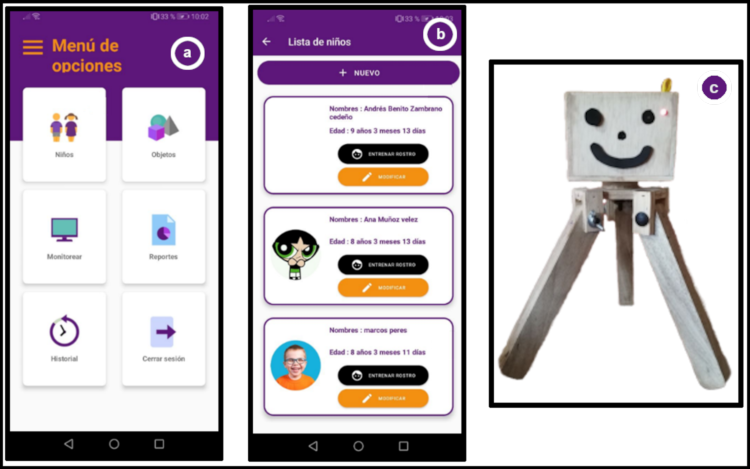
\includegraphics[width=\linewidth]{figs/Figure_9}
                    \caption{Screenshots of the mobile application and the Torddis system device.\label{fig:TorddisApp}} 
                \end{figure}
                
                

\section{Maintenance Plan for the Torddis System}
\label{sup:maintenance}
This supplementary section describes the preventive-maintenance plan devised for the Torddis prototype and the expected service life of its hardware components.

\subsection{Maintenance}
                This phase has not yet been executed due to the limited timeframe required for the development of each deliverable, as well as the time allocated for the overall evaluation of the project. Nevertheless, the system must be maintained in accordance with the preventive guidelines and the expected lifespan of each of its components, in order to ensure proper functionality. Table \ref{tab:maintenance-tasks} outlines some of the potential maintenance tasks. As indicated, each maintenance task—depending on its nature—should be carried out either on a quarterly or semiannual basis, although the actual frequency may vary depending on the operational environment in which the system is deployed.
                
                
                \begin{table}[!htbp]
                    \centering
                    \caption{Definition of selected maintenance tasks.}
                    \label{tab:maintenance-tasks}
                    \begin{tabularx}{\textwidth}{cXcc}
                        \toprule
                        \textbf{No.} & \textbf{Maintenance Tasks} & \textbf{Quarterly} & \textbf{Semiannually} \\
                        \midrule
                        1 & Internal cleaning of the device. & * & \\
                        2 & Check whether the device components exhibit any imperfections or damage. & & * \\
                        3 & Inspect cable connections, condition of cables, connectors, etc. & & * \\
                        4 & Test the operation of the buzzer and LEDs. & * & \\
                        5 & Test the functionality of the computing system (web application server, web services, mobile application, IoT device). & & * \\
                        \bottomrule
                    \end{tabularx}
                \end{table}
                
                Preventive maintenance schedules are defined based on the specific component and its expected service life. Likewise, corrective maintenance for each physical component of the system should be performed before the end of its operational lifespan. The expected service life of each component is presented in Table~\ref{tab:ShelfLife}. The lifespan of resistors is expected to exceed that of the component with the highest durability in the system.
                
                \begin{table}[!htbp]
                    \centering
                    \caption{Service life of the hardware components used in Torddis.}
                    \label{tab:ShelfLife}
                    \begin{tabularx}{\textwidth}{
                            >{\raggedright\arraybackslash}p{2.5cm}
                            >{\raggedright\arraybackslash}X
                            >{\raggedright\arraybackslash}X}
                        \toprule
                        \multicolumn{1}{>{\centering\arraybackslash}p{2.5cm}}{\textbf{Component}} & 
                        \multicolumn{1}{>{\centering\arraybackslash}X}{\textbf{Service Life (years)}} & 
                        \multicolumn{1}{>{\centering\arraybackslash}X}{\textbf{Conditions That Reduce Service Life}}\\
                        
                        \midrule
                        ESP32-CAM & 20 \citep{Espressif2022ESP32-CAM} & Exposure to extreme temperatures, high humidity, dust, or mechanical vibrations.\\
                        
                        ESP8266 Node MCU & 20.83 \citep{Amri2018Improving} to 57 \citep{Ardumotica2023,Espressif2018ESP32Forum} & Extreme temperatures, high humidity levels, dust, voltage spikes, power supply noise, frequent power cycling, intensive WiFi usage at maximum power, firmware updates.\\
                        
                        Passive Buzzer & 3 \citep{HuawhaElectronics} & Excessive voltage, overcurrent, extreme temperatures, vibrations or mechanical shocks, moisture or corrosion, prolonged continuous operation. \\
                        
                        LEDs & 3 \citep{Casamayor2015} to 14 \citep{ShenzhenCary2024LED,GreenLighting2024} & Component degradation, manufacturing conditions. \\
                        
                        Resistors and others & $\infty$ (expected) & High voltage stress \citep{Simon2017Evolution}. \\
                        \bottomrule
                    \end{tabularx}
                \end{table}
                
                The estimation of the components’ service life has been primarily based on references from scientific literature. However, in the absence of relevant academic sources, the specifications provided by manufacturers and distributors have been considered, supplemented in certain cases with information obtained from specialized forums.
                
                